\documentclass[../root.tex]{subfiles}

\begin{document}

\section{Introduction}

\subsection{Overview}

Industrial \emph{robots} are programmed to perform highly specialized and
repetitive actions in controlled environments. Therefore, their
autonomy is quite limited and they are restricted to a small set of
problems. We would like that robots that are
not in such controlled scenarios are able solve a larger variety of
problems, and even to react in the presence
of adverse events.
In other words, we
would like robots to reason about its environment and about the
potential effects that their actions may exert on it.
Such capabilities would allow for great flexibility in the following
ways: (1) tasks can be switched without reprogramming; (2) multiple
solutions to the same problem can be found and assessed in terms
of risk and potential gains in execution speed or other criteria; and (3)
contingency mechanisms can be applied, should adverse events hinder
the execution of the task.

We see in the area of \emph{Automatic Planning and Scheduling},
or simply planning, tools that potentially bring us toward these
desirable qualities.
Planning it is a branch inside Artificial
Intelligence that aims at solving problems that are defined
declaratively, with as little control (procedural) knowledge
as possible.
That is, a
planning algorithm
operates with a model that encodes the dynamics of the domain and, for
each problem, outputs
an action sequence
or a policy that solves it, has a high success probability or has a high
expected reward.

Since Automatic Planning deals with optimizing an agent's
behavior to operate in a certain environment, it is possible to see some
similarities between planning and Reinforcement Learning. The main difference
is that, in their most basic form, a Reinforcement Learning agent is
model-free and dependent on its learning capabilities to decide the
suitable action for a certain state, while a planner takes advantage of a
model of the domain and employs informed search or other heuristic methods to
find a plan (although definitively there
exist works that allow partial domains and that incorporate learning
capabilities to complete these them~\cite{martinez2017relational, martinez2015vmin}).

It is worth saying that planning is not a discipline that is particular to
robotics and, therefore, there exist multiple benchmarks and work in the
field that is general enough to be of use in many areas. One of the
most successful conferences that spreads knowledge in the field of planning is
ICAPS (International Conference in Automatic Planning and Scheduling)
\footnote{\url{http://www.icaps-conference.org/}}. The conference is
held every year and hosts a competition that seeks to push the boundaries
of the state of the art planning systems.

We can think of several applications that are potential targets
of these advances: assistance of old or impaired people for household chores
or treatment~\cite{canal2018adapting,andriella2018deciding}; automatic system
maintenance in difficult-to-access environments, like
subaquatic facilities~\cite{palomeras2016toward,ong2010planning}; and the one
in which we focus on: to \emph{automatically disassembly} electronic devices,
retrieving their most valuable components.

\subsection{Domain of application}

The research presented in this document has been conducted aiming at
developing techniques that can be effectively employed to \emph{recycle}
contraptions such as hard drives, hair trimmers, remote controls or
electronic toys. Fig.~\ref{fig:examples-of-devices} shows some
examples of the devices that we would like to disassemble.

\begin{figure}[tbhp]
	\centering
	\begin{subfigure}[b]{0.31\columnwidth}
		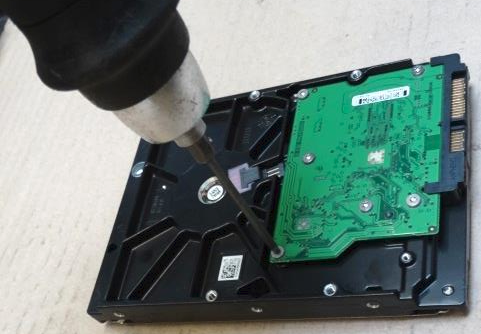
\includegraphics[width=\textwidth]{hddbottom}
		\caption{}
	\end{subfigure}
	~
	\begin{subfigure}[b]{0.31\columnwidth}
		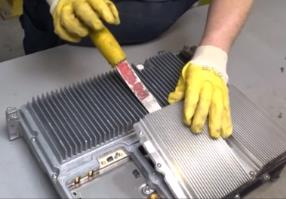
\includegraphics[width=\textwidth]{gsmamp}
		\caption{}
	\end{subfigure}
	~
	\begin{subfigure}[b]{0.31\columnwidth}
		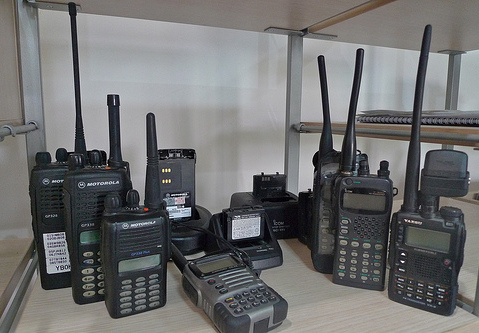
\includegraphics[width=\textwidth]{handies}
		\caption{}
	\end{subfigure}
	\caption{
		(a) Bottom view of a hard drive being disassembled.
		(b) GSM amplifier being disassembled.
		(c) Several handie-talkie models being displayed.
	}
	\label{fig:examples-of-devices}
\end{figure}

In our view, this application poses very attractive challenges
from a scientific point of view. In real-life, deterministic environments
(i.e. fully observable state variables and non-random action outcomes)
are more an exception than a rule, and this becomes evident in disassembly
scenarios. On the one hand, the whole structure of the device cannot be
perceived at once because of occlusions and perception noise, as
Fig.~\ref{fig:examples-of-devices} illustrates. Therefore, progression
in the disassembly task is required to discover hidden components and
geometrical relations. On the other hand, actions might not produce
always the same outcome, due to positioning errors, noise in the movement
of the robots and exogenous factors. For instance, levering the PCB
of a hard drive in order to extract it from the case might not success
entirely, leaving the PCB hovering over one of the edges of the case.
In such case, one may need to consider an additional action like levering
from a different point or holding the case upside down to let the loosen
component fall.

\begin{figure}[tbhp]
	\centering
	\begin{subfigure}[b]{0.48\columnwidth}
		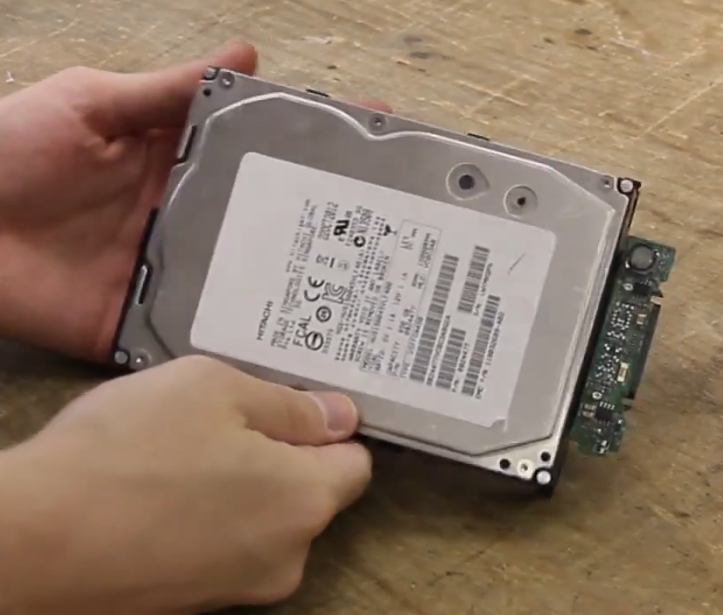
\includegraphics[width=\textwidth]{hddtopcover}
		\caption{}
	\end{subfigure}
	~
	\begin{subfigure}[b]{0.48\columnwidth}
		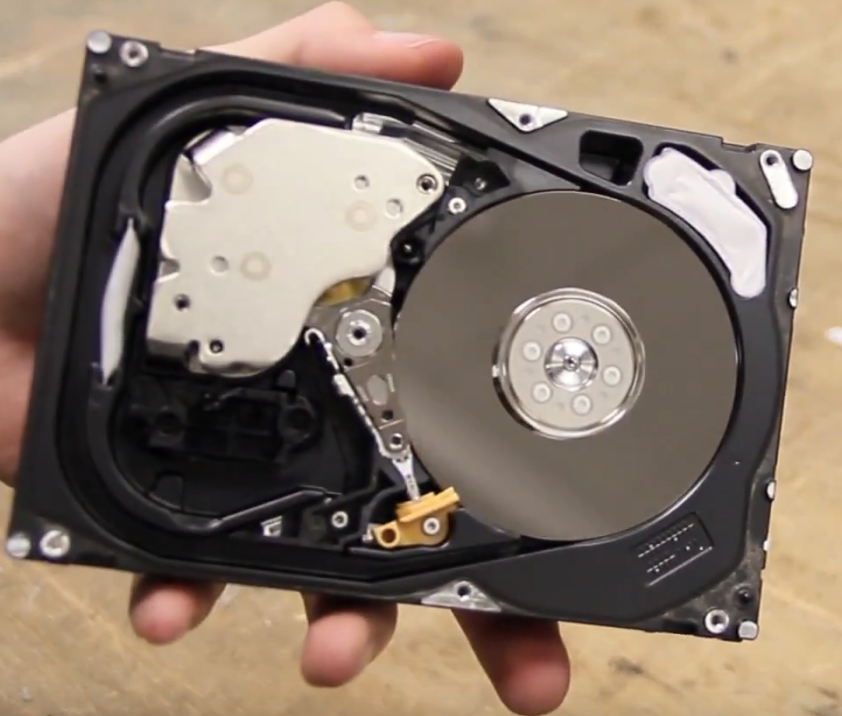
\includegraphics[width=\textwidth]{hddtopwocover}
		\caption{}
	\end{subfigure}
	\caption{
		(a) Top view of a hard drive with the lid.
		(b) View from the same perspective without the lid. The
		previously occluded inner components are now visible.
	}
	\label{fig:example-of-occlusion}
\end{figure}

We cannot forget either the social and environmental impact of the
proposed application. The current recycling industry is dominated
by the \emph{crush and separate} paradigm. Trash is crushed into
very small bits that are then filtered and classified using
physical properties such as density or inductance. However,
the uniformity of the separated debris cannot be guaranteed.
Even more importantly, devices often contain components or
substances that are hazardous for the environment. In such cases,
it is require that a human manually removes the source of danger.
This has associated health risks for the operator. Moreover,
it is inefficient and costly, so a great amount of trash is
simply incinerated, posing a serious thread for the ecosystems.
Another drawback of this method is that precious or reusable
components (e.g. PCBs, capacitors, magnets...) are destroyed,
when they can be used right away or after some refurnishing
in the manufacturing of new products.

In light of these arguments, a robotic recycling system is
appealing from a sustainability point of view.
To solve the previously exposed drawbacks, we would like
the following features: (1) the robot should
ideally adapt to different electromechanical contraptions
(including different brands/models of the same device);
(2) the robot should correctly identify the tasks that it
has to complete to perform a successful disassembly; and (3)
it should be able to work even with damaged devices.

\section{Involvement in H2020 Imagine}

\section{Scope and goals}

\section{Related work}

\IfEq{\jobname}{\detokenize{root}}{}{\printbibliography}

\end{document}